\documentclass[WHATMANUAL.tex]{subfiles}

\begin{document}

\chapter{Hydrogeological characterization of the containment level of the regional bedrock aquifer in Monteregie Est}

\section{Introduction}

Des hydrogrammes de puits ont été enregistrés dans quatre puits d’observation existants et les 44 puits installés dans le cadre du projet PACES en Montérégie Est. Les hydrogrammes dans les puits nouvellement installés ont des durées d’enregistrement de l’ordre de deux ans. La grande majorité des puits d’observation ont été installés dans l’aquifère rocheux fracturé régional. En plus de pouvoir être utilisés pour évaluer la recharge, les hydrogrammes de puits peuvent aussi donner des indications sur les conditions de confinement de l’aquifère rocheux régional, selon leurs variations saisonnières par rapport aux périodes de recharge de la nappe. C’est ce qui est décrit dans la présente section.

Les données météorologiques (température et précipitations) ont été compilées et mises en relation avec les hydrogrammes de puits disponibles (voir Annexe x pour la compilation des hydrogrammes de puits). Le comportement relatif des hydrogrammes de puits, particulièrement durant les périodes de recharge, a été utilisé pour regrouper les hydrogrammes en classes de comportements. Ces classes sont interprétées en termes de conditions de confinement de l’aquifère rocheux régional. Les indications de confinement déduites des hydrogrammes sont comparées à la carte régionale des conditions de confinement basée sur de la séquence et l’épaisseur des dépôts meubles. Les hydrogrammes fournissent ainsi une validation indépendante des critères utilisés pour définir les conditions de confinement de l’aquifère rocheux régional.

\section{Données météorologiques}

Les données météorologiques journalières (température maximale, minimale et moyenne ainsi que les accumulations sous forme de pluie et de neige) de 32 stations météorologiques situées à l'intérieur et autour de la Montérégie Est ont été récupérées sur le site d'Environnement Canada pour la période allant du 1er janvier 2000 au 31 décembre 2012. Cette période englobe celle des enregistrements des hydrogrammes pour les nouveaux puits d’observation installés en Montérégie Est dans le cadre du projet PACES. Des polygones de Thiessen ont été générés à partir de la localisation de ces 32 stations. Chacun des puits d'observation situés en Montérégie Est a par la suite été associé à une station météorologique (voir figure 1). Lorsqu'un puits était situé très près d'une limite entre deux polygones de Thiessen, la station météorologique dont l'altitude était la plus similaire à celle du puits a été sélectionnée (ex.: PO10 et PO16). 

De ces 32 stations météorologiques, un total de 18 stations ont été associées à au moins un puits d'observation. Les données manquantes de chacune de ces 18 stations ont été comblées de façon automatique à l'aide d'une routine rédigée dans Matlab. La méthode consiste à construire, pour chacune des données manquantes, un modèle de régression linéaire multiple entre la station traitée et les stations voisines les mieux corrélées dont des données sont disponibles. Cette approche a été identifiée par Xia et al. (1999) et Eischeid et al. (2000) comme étant l'une des méthodes les plus performantes pour l'estimation de données météorologiques manquantes parmi celles couramment utilisées dans le domaine. Les détails de la méthode seront donnés dans la thèse de doctorat de Jean-Sébastien Gosselin.

\begin{figure}
\centering
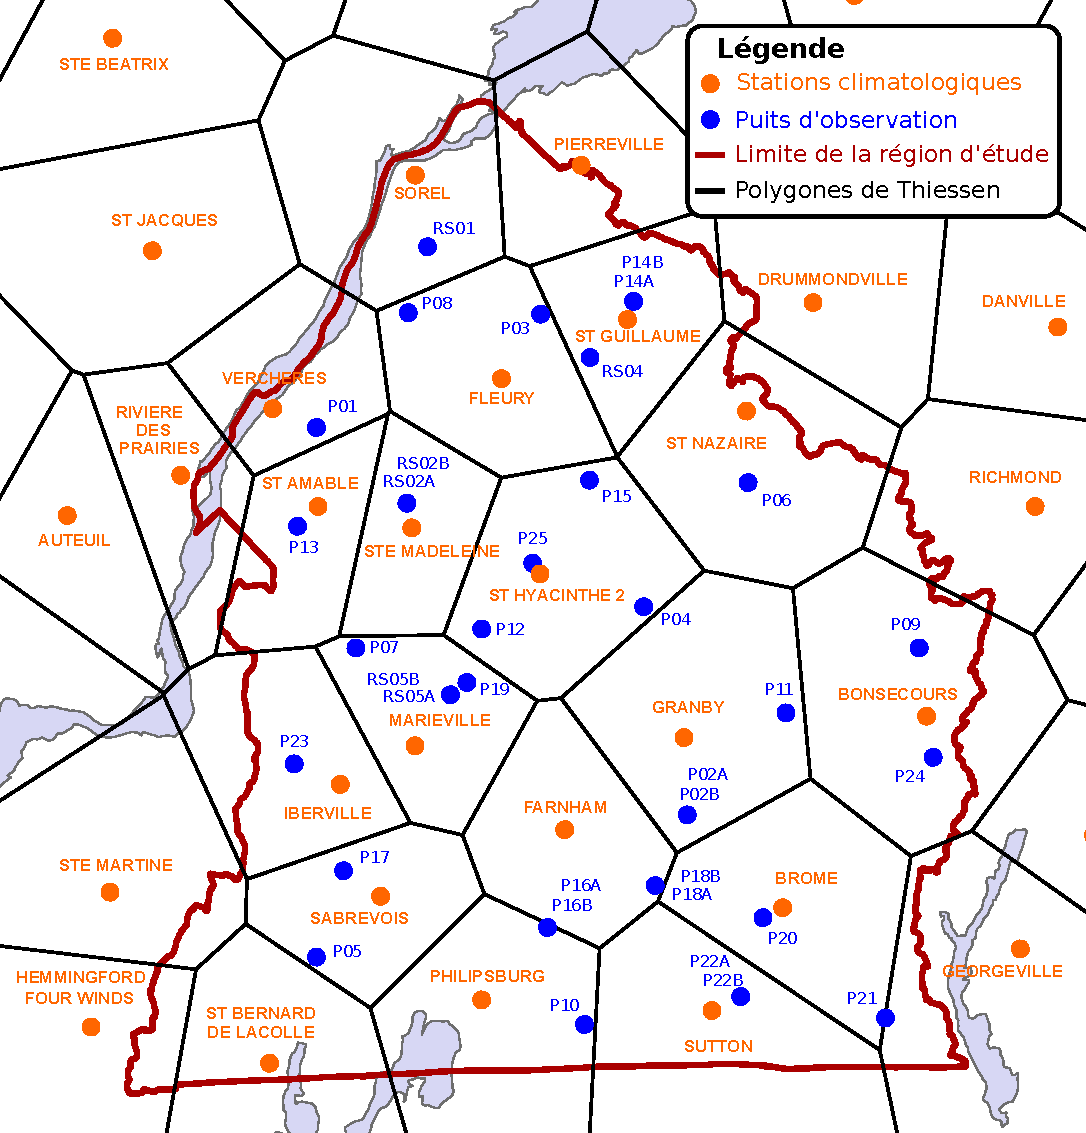
\includegraphics[width=0.75\textwidth]{img/Thiessen_meteo_wells}
\caption[Conditions de confinements déduites des hydrogrammes de puits (points) par rapport à la carte des conditions de confinement de l’aquifère rocheux régional.]{Localisations des puits d’observation (points verts) et des stations météorologiques (points noirs). Les polygones de Thiessen permettent d’assigner une station météorologique aux puits d’observation.}
\label{fig:tab_hydrograph_layout}
\end{figure}

\section{Hydrogrammes de puits et conditions de confinement}

Des graphiques d'hydrogrammes de puits ont été générés à partir des niveaux d'eau mesurés dans un total de 44 puits d'observation sur la période allant de novembre 2010 à novembre 2012 (tableau x). Ces graphiques contiennent les niveaux d'eau tracés aux 6 h et exprimés en profondeur (m) sous la surface du sol et des histogrammes des précipitations totales hebdomadaires (pluie et neige en équivalent en eau) et des températures maximales moyennes hebdomadaires. La température et les précipitations ont été tracées sur une base hebdomadaire car ce format facilite l'interprétation visuelle des données. Les figures ont été produites de façon automatisée à l'aide d'une routine rédigée dans Matlab.

Les variations de niveau d'eau enregistrées lors des événements de précipitations et de fonte ont été interprétées qualitativement et chacun des hydrogrammes a été classé selon trois groupes en fonction de leur comportement. Sur la base de ces observations, les conditions de confinement de l’aquifère rocheux régional ont pu être déduites à 35 sites au total puisqu’un certain nombre des 44 puits sont multi-niveaux et situé côte-à-côte à la même localisation. Les conditions de confinement ont été définies en trois classes: (1) libre, (2) captif et (3) semi-captif ou captif avec influence régionale. La figure 2 montre des hydrogrammes typiques des comportements reliés aux différentes conditions de confinement.

À des fins de comparaison, les résultats des interprétations basées sur les hydrogrammes ont été reportés sur la carte des conditions de confinement de l’aquifère rocheux régional qui a été produite en fonction de l'épaisseur et de la nature des dépôts meubles (figure 3). Lorsque seulement des mesures de niveau d’eau étaient disponibles dans les dépôts meubles et non dans le roc (ex.: Farnham, Saint-Alexandre, Sainte-Christine, Saint-Paul-d'Abbotsford et Saint-Alphonse), les interprétations découlant de ces données ont été indiquées avec des symboles différents sur la carte (avec des carrés plutôt que des cercles).

La figure 3 montre que les conditions de confinement de l’aquifère rocheux régional définies sur la base des hydrogrammes de puits sont de façon générale très cohérentes avec celles de la carte des conditions de confinement. Ce résultat est particulièrement intéressant, considérant que les deux approches sont indépendantes. Ainsi, la définition des conditions de confinement de l’aquifère rocheux pour les deux approches découle de critères basés sur des quantités physiques qui sont de nature très différentes: série temporelle de niveaux piézométriques dans un cas et distribution spatiale des dépôts meubles dans l'autre. Les conditions de confinement déduites des hydrogrammes de puits viennent ainsi valider les critères utilisés pour produire la carte régionale des conditions de confinement. Ces critères ont été basés sur un jugement professionnel et ils sont donc relativement arbitraires, même s’ils sont logiques en fonction des conditions régionales.

\begin{figure}
\centering
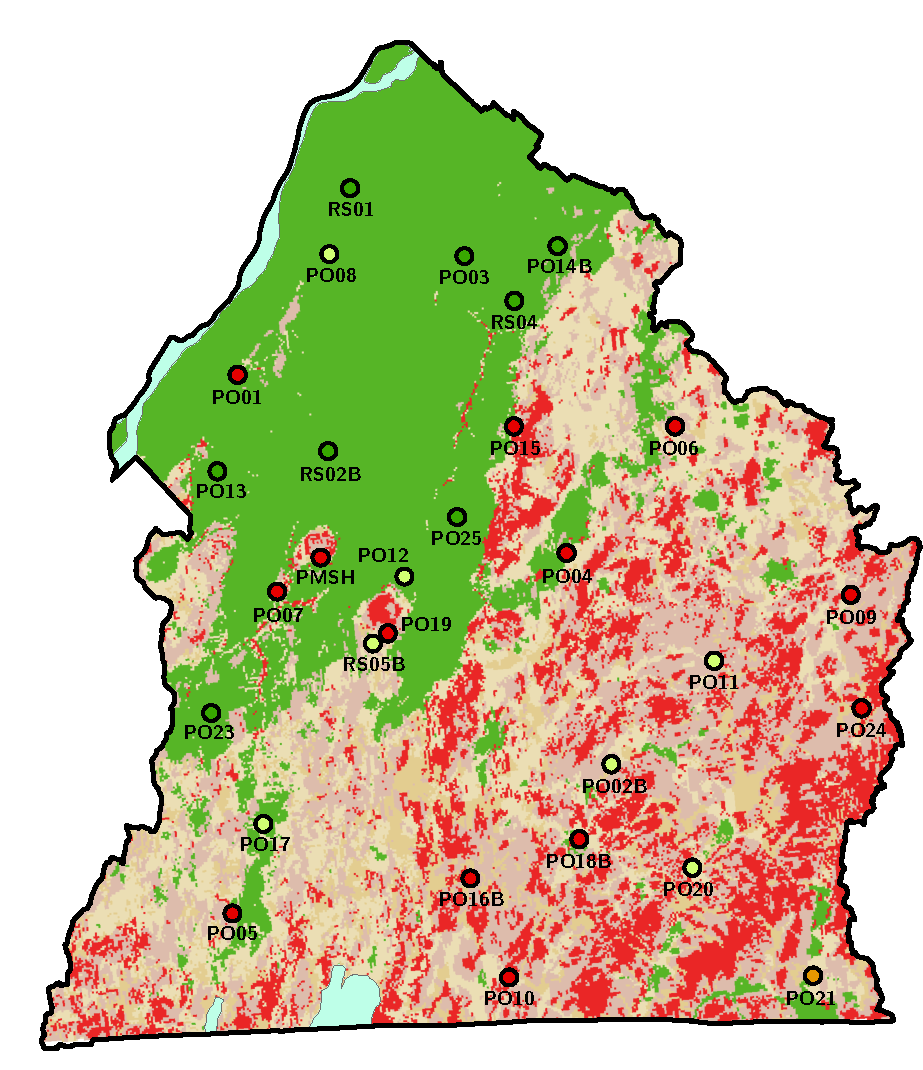
\includegraphics[height=0.85\textheight]{img/CONFINEMENTetPUITS}
\caption[Conditions de confinements déduites des hydrogrammes de puits (points) par rapport à la carte des conditions de confinement de l’aquifère rocheux régional.]{Conditions de confinements déduites des hydrogrammes de puits (points) par rapport à la carte des conditions de confinement de l’aquifère rocheux régional. Les cercles représentent des puits au roc et les carrés des puits dans les dépôts meubles. Les couleurs indiquent les conditions de confinement, tant pour la carte que les symboles pour les puits : vert pour captif, rouge pour libre et autres tons pour semi-captif.}
\label{fig:tab_hydrograph_layout}
\end{figure}

De façon globale, les résultats obtenus avec les hydrogrammes de puits sont également cohérents avec les différents contextes hydrogéologiques définis en Montérégie Est. On retrouve les puits d’observation jugés représentatifs de conditions captives exclusivement dans les Basses-terres, principalement dans la partie nord de la région où on retrouve une grande épaisseur d’argile. De plus, les hydrogrammes donnent des indications du confinement pour des zones plus locales. Par exemple, le puits PO01 représente bien la zone de recharge locale située dans la partie nord-ouest des Basses-terres, où l'on retrouve des dépôts meubles moins épais et ayant une texture plus grossière. On note également que le puits PO08, situé à environ 20 km de PO01 et à moins de 7 km de la limite de cette zone de recharge, présente des variations saisonnières de la piézométrie qui sont importantes (de 1 à 2 m de 2010 à 2012) en dépit de l'épaisse couche d'argile (plus de 25 m) qui recouvre le roc à cet endroit. Il est possible que ces variations du niveau piézométrique au puits PO08 soient causées par une influence provenant de la zone de recharge du roc située à proximité. La partie sud des Basses-terres est caractérisée quant à elle par des puits reflétant des conditions captives, semi-captives et libres qui sont distribuées de façon cohérente avec la carte des conditions de confinement.

Le Piémont appalachien est caractérisé par des puits indiquant exclusivement des conditions libres. Plus spécifiquement, le puits PO18 situé dans une petite cuvette du roc dans le sud du Piémont est particulièrement intéressant. Malgré que le roc soit recouvert de plus de 40 m de dépôts meubles à cet endroit, on observe que les variations du niveau d'eau dans le puits sont fortement corrélées avec les précipitations et la fonte printanière, indiquant des conditions libres. 
Ceci suggère que l'aquifère rocheux régional dans la cuvette est fortement connecté à l'aquifère rocheux libre à semi-captif retrouvé tout autour de la cuvette. Il est intéressant de voir comment il est possible d'utiliser la carte de confinement  du roc comme un outil pour expliquer le comportement de la piézométrie mesurée dans les puits d'observation.

Les Hautes-terres appalachiennes sont caractérisées par des puits indiquant des conditions allant de libres à semi-captives. Ces résultats représentent bien la couverture discontinue des dépôts meubles dans ce contexte hydrogéologique. Le fait que l'on ne retrouve pas de puits indiquant des conditions captives, malgré des épaisseurs de dépôts meubles parfois importantes dans les vallées, incluant des sédiments fins, suggère une influence significative des zones de recharge de l’aquifère rocheux situées en élévation sur les zones située dans les creux topographiques (vallées). Le puits PO20, classé comme ayant un comportement de type semi-captif et montrant plus de 24 m de dépôts, est un bon exemple.

Les puits localisés sur ou près des Montérégiennes représentent également bien ce que l'on retrouve sur la carte des conditions de confinement de l’aquifère rocheux régional. On remarque que les puits indiquent des conditions libres sur les Montérégiennes et des conditions qui varient entre libres et semi-captives au pourtour de celles-ci. Cela est particulièrement bien représenté par les puits PO19, PO12 et RS05b situés dans les environs du Mont Rougemont : le puits PO19, situé directement sur le Mont Rougemont, indique des conditions libres, alors que les puits PO12 et RS05b ont une réponse indiquant des conditions semi-captives. Ce comportement est particulièrement surprenant pour le puits PO12 où le roc est recouvert par une épaisse couche de silt argileux de plus de 23 m. Ceci pourrait être un indicateur de l'étendue de l'influence de la recharge de l’aquifère rocheux par les Montérégiennes. Ces collines sont effectivement considérées comme étant des zones de recharge préférentielle dans la région et ces données semblent suggérer qu’elles pourraient même avoir une influence sur la piézométrie de l’aquifère rocheux à une certaine distance des Montérégiennes, où l’aquifère rocheux peut être recouvert par d'importantes épaisseurs de sédiments fins.

\section{Discussion}

L'interprétation qualitative de la réponse des niveaux d'eau aux événements de précipitations et de fonte a permis de valider l’évaluation des conditions de confinement basée sur l’épaisseur et la nature des dépôts meubles. Néanmoins, le classement du comportement des puits demeure qualitatif. En réalité, le niveau de confinement de l’aquifère rocheux n'est pas clairement défini en trois classes bien distinctes, mais varie plutôt sur une gamme continue de comportements indiquant des conditions allant de parfaitement libres à parfaitement captives. Le classement des puits est d'autant plus difficile considérant la période relativement courte (2 ans ou moins) sur laquelle des données de niveaux d’eau sont présentement disponibles pour la majorité des puits. Ainsi, une mise à jour de l’interprétation des hydrogrammes et une vérification des résultats devrait être réalisée lorsque la période de mesures sera plus longue (au moins 5 ans).  

Il est à noter que des données de niveaux d'eau dans tous les puits d'observation de la Montérégie à une fréquence de 15 minutes seront bientôt disponibles de décembre 2012 jusqu'à avril ou mai 2013. Ces données à haute résolution temporelle permettront de quantifier le niveau de captivité des aquifères par des analyses de la réponse des puits aux variations de la pression atmosphérique. Cette approche a déjà donné des résultats prometteurs dans quelques autres projets de recherche en hydrogéologie (Rasmussen et Crawford, 1996; Butler et al., 2011). Il sera intéressant d'appliquer ces nouveaux concepts aux contextes hydrogéologiques retrouvés en Montérégie Est.

\end{document}